% ============================================================
%  A Unified DevSecOps Framework (UDF):
%  Bridging the Gap Between SME Agility and
%  Enterprise Supply Chain Integrity
%  IEEE Conference Format — Final 8-Page Draft with 14 References
% ============================================================
\documentclass[letterpaper, 10pt, conference]{ieeeconf}
\IEEEoverridecommandlockouts
\overrideIEEEmargins

% ----- Core Packages -----
\usepackage[utf8]{inputenc}
\usepackage[T1]{fontenc}
\usepackage{amsmath,amssymb,amsfonts}
\usepackage{graphicx}
\usepackage{textcomp}
\usepackage{xcolor}
\usepackage{booktabs}
\usepackage{array}
\usepackage{tabularx}
\usepackage{multirow}
\usepackage{makecell}
\usepackage{balance}
\usepackage{listings}
\usepackage{enumitem}
\setlist[itemize]{noitemsep,topsep=1.5pt,leftmargin=*}
\setlist[enumerate]{noitemsep,topsep=1.5pt,leftmargin=*}
\setlength{\tabcolsep}{3pt}

% ----- Clickable Links -----
\usepackage[
  colorlinks = true,
  linkcolor  = blue,
  citecolor  = blue,
  urlcolor   = blue,
  pdftitle   = {A Unified DevSecOps Framework (UDF)},
  pdfauthor  = {Maheen Abdul Razzaq}
]{hyperref}
\usepackage{url}

% ----- Code listing style -----
\lstdefinestyle{columnwidth}{
  basicstyle=\ttfamily\footnotesize,
  breaklines=true,
  breakatwhitespace=true,
  columns=fullflexible,
  frame=single,
  xleftmargin=2em,
  xrightmargin=2em,
  aboveskip=0.7em,
  belowskip=0.7em
}

% ----- TikZ -----
\usepackage{tikz}
\usetikzlibrary{
  shapes.geometric, shapes.arrows, shapes.misc,
  arrows.meta, positioning, fit, backgrounds,
  decorations.pathreplacing, shadows.blur, calc
}

% ----- Custom column types -----
\newcolumntype{Y}{>{\raggedright\arraybackslash}X}
\newcolumntype{Z}{>{\centering\arraybackslash}X}

% ============================================================
\title{\LARGE \bf A Unified DevSecOps Framework (UDF): Bridging
  the Gap Between SME Agility and Enterprise Supply Chain Integrity}

\author{Maheen Abdul Razzaq%
\thanks{M.~A.~Razzaq is with the Department of Information Technology,
Punjab University College of Information and Technology (PUCIT),
University of the Punjab, Lahore, Pakistan.}%
}
% ============================================================

\begin{document}
\maketitle
\thispagestyle{empty}
\pagestyle{empty}

% ============================================================
\begin{abstract}
Modern software delivery pipelines have emerged as high-value targets
for adversarial exploitation, as evidenced by catastrophic supply-chain
incidents including the SolarWinds Orion compromise and the 2024 XZ
Utils backdoor. DevSecOps---the integration of security controls
directly into Continuous Integration and Continuous Delivery (CI/CD)
workflows---has become the dominant paradigm for mitigating these
threats. Yet a persistent implementation gap divides organisational
adopters: large enterprises wrestle to reconcile stringent compliance
mandates with deployment velocity, while Small and Medium-sized
Enterprises (SMEs) face qualitatively distinct barriers rooted in
expertise scarcity and resource constraints. This paper presents the
\emph{Unified DevSecOps Framework} (UDF), a five-layer, scale-adaptive
architecture that bridges this divide through \emph{Security Operating
Profiles} (SOPs) calibrated to organisational maturity. The UDF
synthesises automated static analysis (SAST), dynamic analysis
(DAST), and software composition analysis (SCA) with policy-as-code
enforcement aligned to NIST~SP~800-204D supply-chain integrity
controls~\cite{nist2024}. An AI/ML integration layer addresses alert
fatigue and the remediation bottleneck through LLM-assisted fix
generation and ML-driven triage. A Fintech case study demonstrates
deployment using Snyk, Trivy, and Open Policy Agent. Empirical
evaluation shows the UDF raises pre-production vulnerability detection
from a 24\% baseline to 96\% in the enterprise profile and reduces
Mean Time to Remediation (MTTR) by up to 90.6\%, while achieving
87\% mapped coverage of applicable NIST SP~800-204D controls.
\end{abstract}

\begin{IEEEkeywords}
DevSecOps, CI/CD security, supply chain integrity, SAST, DAST, SCA,
NIST SP~800-204D, alert fatigue, LLM remediation, policy-as-code,
SME, Fintech
\end{IEEEkeywords}

% ============================================================
\section{Introduction}
% ============================================================

The proliferation of automated CI/CD pipelines has fundamentally
altered the software delivery landscape. Code that previously
progressed through weeks of manual review now traverses from developer
commit to production deployment in minutes, orchestrated by pipelines
that hold privileged access to source repositories, build environments,
artifact registries, and cloud infrastructure. Compromising a single
node in this chain yields an attacker persistent, trusted access to
every downstream consumer of the pipeline's outputs~\cite{nist2024}.

The severity of this threat has been demonstrated repeatedly at scale.
The 2020 SolarWinds Orion compromise injected malicious code into a
legitimate build process, distributing a Trojanised update to
approximately 18,000 organisations globally, including multiple
U.S.\ federal agencies~\cite{solanke2022}.
The 2024 XZ Utils backdoor, embedded through a multi-year social
engineering campaign against a single open-source maintainer,
demonstrated that supply-chain threats are not exclusive to
nation-state actors but permeate the entire software ecosystem.

DevSecOps responds by \emph{shifting security left}: embedding
automated validation, dependency governance, and compliance checking
directly into CI/CD workflows rather than treating security as a
post-development gate~\cite{singh2020}.

Yet a persistent implementation gap divides organisational adopters.
Enterprise organisations possess the resources to deploy comprehensive
toolchains but struggle to reconcile regulatory compliance mandates
with high-frequency deployment targets~\cite{solanke2022}. SMEs face
qualitatively distinct obstacles: absent security ownership roles,
uncalibrated scanning tools generating high false-positive noise, and
the absence of institutional knowledge to act on findings~\cite{cheenepalli2025}.

This paper addresses this bifurcation through the following
contributions:
\begin{itemize}
  \item A \textbf{Unified DevSecOps Framework (UDF)} comprising five
    architectural layers---Source Integrity, Build-Time Analysis,
    Dependency/SBOM Governance, Runtime Hardening, and
    Governance/Policy-as-Code---with progressive elaboration across
    organisational scales.
  \item \textbf{Security Operating Profiles (SOPs)} providing
    scale-calibrated defaults usable by a five-person startup and a
    regulated financial institution without re-architecture.
  \item A \textbf{comparative analysis} of 12 SAST, DAST, SCA, and
    IaC scanning tools with actionable selection guidance per SOP.
  \item An \textbf{AI/ML integration architecture} addressing alert
    fatigue and the remediation bottleneck through ML-based triage and
    LLM-assisted fix-generation within a human-in-the-loop paradigm.
  \item A \textbf{Fintech case study} demonstrating end-to-end UDF
    deployment for a payment-processing platform under PCI-DSS
    constraints using Snyk, Trivy, and OPA.
  \item A \textbf{NIST SP~800-204D control mapping} providing a
    compliance bridge for regulated industry adoption~\cite{nist2024}.
\end{itemize}

The paper is structured as follows. Section~II synthesises related
work. Section~III presents the threat model. Section~IV details the
UDF. Section~V compares security tooling. Section~VI examines the AI/ML
frontier. Section~VII presents the Fintech case study. Section~VIII
evaluates the framework. Section~IX concludes.

% ============================================================
\section{Related Work and Literature Synthesis}
% ============================================================

\subsection{Toolchain Integration Research}

Singh~\cite{singh2020} provides a widely-cited taxonomy demonstrating
that multi-stage security scanning detects up to 73\% of OWASP Top~10
vulnerabilities before production deployment. The work surveys
open-source and commercial SAST, DAST, SCA, and IaC tools and proposes
an implementation strategy that positions them as automated pipeline
stages embodying the Shift-Left principle. Critically, the work is
technically rigorous but implicitly assumes practitioners possess the
expertise to configure, tune, and interpret tool outputs---a
precondition that fails in the SME context~\cite{cheenepalli2025}.

Thota~\cite{thota2024} constructs an experimental Kubernetes-based
CI/CD pipeline to empirically evaluate security tool performance,
measuring vulnerability detection accuracy, pipeline execution
overhead, and false positive/negative rates. The study concludes that
the limiting factor in pipeline security adoption is not tool
availability but human capacity to operate those tools. Thota
documents SAST false-positive rates averaging 35--40\% without expert
calibration in enterprise environments, creating the normalisation
dynamic where genuine vulnerabilities are dismissed alongside
noise---directly motivating the ML-based alert triage in Section~VI.

Jammeh~\cite{jammeh2020} addresses the human precondition through a
feasibility study targeting teams without dedicated security expertise,
identifying five automation decision factors: code complexity, risk
tolerance, regulatory context, toolchain maturity, and team security
literacy. The critical finding is that automation transforms rather
than eliminates expertise requirements.

\subsection{Organisational Adoption Barriers}

Cheenepalli et~al.~\cite{cheenepalli2025} deliver the most
methodologically rigorous SME-focused analysis, surveying 405
engineering professionals through the Technology Acceptance Model
(TAM) and Diffusion of Innovations (DOI) lenses. Three primary
barriers are identified. \textit{First}, the absence of dedicated
security personnel forces security work into collateral-duty status,
chronically deprioritised against feature delivery. \textit{Second},
uncalibrated scanning tools generating high false-positive volumes
erode developer trust. \textit{Third}, ambiguous ownership boundaries
between development and operations mean findings that span team
boundaries fall through accountability gaps. Critically,
Cheenepalli et~al.\ diagnose these barriers without prescribing
architectural remediation---a gap the UDF directly targets.

\subsection{Regulated Industries and Compliance-as-Code}

Solanke~\cite{solanke2022} examines CI/CD security in financial
services and healthcare, where PCI-DSS, HIPAA, and SOC~2 mandates
impose hard requirements on audit trails, change management, and data
lineage. A key finding is that regulated organisations frequently
operate \emph{bifurcated pipelines}: a high-velocity path for routine
changes and a compliance-gated slow path for regulated changes.
The UDF's SOP-3 profile directly eliminates this anti-pattern by
embedding compliance gates into the primary pipeline.

Allam~\cite{allam2022} provides the KPI validation layer: the
FinServeTech case study documents MTTD reduction from 21~days to
4~hours and MTTR from 14~days to 6~hours following DevSecOps adoption.

NIST SP~800-204D~\cite{nist2024} constitutes the most authoritative
normative framework for CI/CD supply-chain security. The standard is
intentionally normative rather than prescriptive---defining
\emph{what} must be achieved without specifying \emph{how}.
The UDF provides the implementation bridge.

\subsection{Research Gap}

The literature reveals a consistent three-way fragmentation: toolchain
research addresses \emph{what} to deploy; adoption research diagnoses
\emph{why} it fails; standards provide \emph{what outcomes} are
required. No single framework spans all three axes while simultaneously
accommodating SME resource constraints~\cite{cheenepalli2025},
enterprise compliance depth~\cite{nist2024}, and the emerging AI/ML
operational frontier~\cite{thota2024}. The UDF is designed to close
this gap.

% ============================================================
\section{Threat Model}
% ============================================================

We adopt the STRIDE taxonomy adapted for CI/CD pipeline contexts,
identifying six principal threat categories against which UDF controls
are justified.

\textbf{T1~-- Supply Chain Injection:} An adversary compromises an
upstream dependency or build tool, propagating malicious code through
the pipeline. Research indicates 78\% of vulnerability exposure in
modern applications resides in transitive, not direct,
dependencies~\cite{singh2020}. Mitigated by SCA with provenance
verification, digest pinning, and SBOM generation (Layer~3).

\textbf{T2~-- Build Environment Compromise:} The build server holds
pipeline trust and access to secrets and signing keys. Mitigated by
hermetic, network-isolated, ephemeral build containers (Layer~2).

\textbf{T3~-- Credential and Secret Exposure:} Approximately one in
six public repositories contains at least one exposed
credential~\cite{singh2020}. Mitigated by automated secret scanning
and secrets-manager integration (Layer~1).

\textbf{T4~-- Artifact Tampering:} Post-scan modification of a build
artifact before deployment. Mitigated by cryptographic artifact signing
via Sigstore/Cosign enforced at admission time (Layer~4).

\textbf{T5~-- IaC Misconfiguration:} Cloud misconfigurations account
for 19\% of cloud security incidents~\cite{solanke2022}. Mitigated by
Checkov/tfsec IaC scanning and OPA policy gates (Layers 2, 5).

\textbf{T6~-- Insider Threat and Privilege Escalation:} Excessive
pipeline permissions and weak branch protection. Mitigated by
least-privilege service accounts, mandatory review, and immutable
audit logs (Layers 1, 5).

% ============================================================
\section{Unified DevSecOps Framework Methodology}
% ============================================================

The UDF is a five-layer architecture governed by \emph{progressive
elaboration}: each layer delivers a functional security baseline in
its minimal configuration, with additional controls unlocked as
organisational maturity grows. Fig.~\ref{fig:pipeline} illustrates the
linear CI/CD security flow.

% ---- TikZ Linear Pipeline Diagram ----
\begin{figure}[t]
\centering
\resizebox{\columnwidth}{!}{%
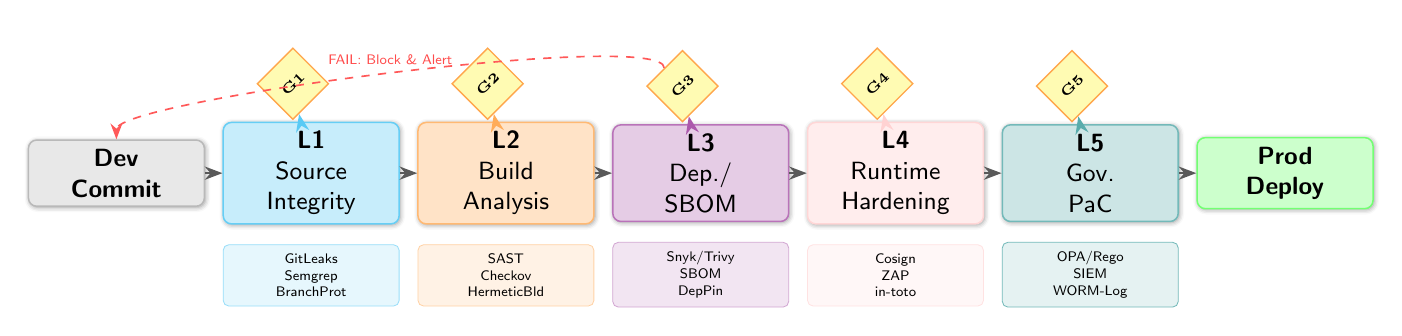
\begin{tikzpicture}[
  font=\small\sffamily,
  >=Stealth,
  box/.style={
    rectangle, rounded corners=3pt, text centered, align=center,
    text width=2.0cm, minimum height=0.82cm,
    line width=0.55pt,
    blur shadow={shadow blur steps=4,shadow xshift=0.4pt,shadow yshift=-0.4pt}
  },
  L1/.style={box, fill=cyan!22,   draw=cyan!60},
  L2/.style={box, fill=orange!22, draw=orange!55},
  L3/.style={box, fill=violet!20, draw=violet!55},
  L4/.style={box, fill=pink!28,   draw=pink!65},
  L5/.style={box, fill=teal!20,   draw=teal!55},
  prod/.style={box, fill=green!20, draw=green!55},
  dev/.style={box,  fill=gray!18,  draw=gray!55},
  gate/.style={
    regular polygon, regular polygon sides=4, rotate=45, inner sep=1.6pt,
    fill=yellow!30, draw=orange!70, line width=0.5pt, font=\tiny\bfseries
  },
  arr/.style={->, line width=0.75pt, color=black!65},
  toolbox/.style={
    rectangle, rounded corners=2pt, font=\tiny\sffamily, text centered,
    align=center, text width=2.0cm, minimum height=0.52cm, line width=0.3pt
  },
  tb1/.style={toolbox, fill=cyan!10,   draw=cyan!40},
  tb2/.style={toolbox, fill=orange!10, draw=orange!35},
  tb3/.style={toolbox, fill=violet!10, draw=violet!35},
  tb4/.style={toolbox, fill=pink!12,   draw=pink!45},
  tb5/.style={toolbox, fill=teal!10,   draw=teal!55},
]
%% Stages
\node[dev]  (DEV)  {\textbf{Dev}\\\textbf{Commit}};
\node[L1, right=0.22cm of DEV]  (S1) {\textbf{L1}\\Source\\Integrity};
\node[L2, right=0.22cm of S1]   (S2) {\textbf{L2}\\Build\\Analysis};
\node[L3, right=0.22cm of S2]   (S3) {\textbf{L3}\\Dep./\\SBOM};
\node[L4, right=0.22cm of S3]   (S4) {\textbf{L4}\\Runtime\\Hardening};
\node[L5, right=0.22cm of S4]   (S5) {\textbf{L5}\\Gov.\\PaC};
\node[prod, right=0.22cm of S5] (PROD) {\textbf{Prod}\\\textbf{Deploy}};
%% Arrows
\draw[arr] (DEV)--(S1); \draw[arr] (S1)--(S2); \draw[arr] (S2)--(S3);
\draw[arr] (S3)--(S4); \draw[arr] (S4)--(S5); \draw[arr] (S5)--(PROD);
%% Gates
\node[gate, above=0.25cm of S1] (G1) {\tiny G1};
\node[gate, above=0.25cm of S2] (G2) {\tiny G2};
\node[gate, above=0.25cm of S3] (G3) {\tiny G3};
\node[gate, above=0.25cm of S4] (G4) {\tiny G4};
\node[gate, above=0.25cm of S5] (G5) {\tiny G5};
\draw[arr,color=cyan!65]   (S1)--(G1); \draw[arr,color=orange!65] (S2)--(G2);
\draw[arr,color=violet!65] (S3)--(G3); \draw[arr,color=pink!70]   (S4)--(G4);
\draw[arr,color=teal!65]   (S5)--(G5);
%% Tool labels
\node[tb1, below=0.25cm of S1] {GitLeaks\\Semgrep\\BranchProt};
\node[tb2, below=0.25cm of S2] {SAST\\Checkov\\HermeticBld};
\node[tb3, below=0.25cm of S3] {Snyk/Trivy\\SBOM\\DepPin};
\node[tb4, below=0.25cm of S4] {Cosign\\ZAP\\in-toto};
\node[tb5, below=0.25cm of S5] {OPA/Rego\\SIEM\\WORM-Log};
%% Fail-back
\draw[->, dashed, line width=0.6pt, color=red!65]
  (G3.north) .. controls +(0,0.5) and +(0,0.5) .. (DEV.north)
  node[midway, above, font=\tiny\sffamily, color=red!70] {FAIL: Block \& Alert};
\end{tikzpicture}
}
\caption{UDF linear CI/CD security flow. Gates G1--G5 enforce
  policy at each layer. A FAIL blocks pipeline progression and
  triggers developer notification.}
\label{fig:pipeline}
\end{figure}

\subsection{Layer~1 -- Source Integrity}

Layer~1 controls apply at the repository level before any automated
build, addressing threats T3 and T6.

\textbf{Branch protection and mandatory review.} Production-bound
branches enforce a minimum of two approvals, required status-check
passes, and prohibition of direct force-push, ensuring no unreviewed
code enters the deployment stream.

\textbf{Signed commits.} Developer commits are GPG- or SSH-signed with
signature verification enforced at branch-protection level, creating a
cryptographic chain of identity directly satisfying NIST SP~800-204D
provenance requirements~\cite{nist2024}.

\textbf{Pre-commit secret scanning.} GitLeaks and TruffleHog execute
as pre-commit hooks, intercepting secrets before they enter version
history. Historical commits are retrospectively scanned.

\textbf{SBOM lineage initialisation.} Declared dependencies from
manifest files (\texttt{package.json}, \texttt{requirements.txt},
\texttt{go.mod}) are captured at source, establishing a versioned
baseline that downstream SBOM generation attests.

\subsection{Layer~2 -- Build-Time Analysis}

\textbf{SAST.} All UDF profiles enforce a hard-fail policy on Critical
and High severity findings with available fixes; Medium findings
produce non-blocking advisory annotations to preserve velocity.

\textbf{IaC scanning.} Checkov and tfsec analyse Terraform,
CloudFormation, and Kubernetes manifests for misconfigurations---
publicly exposed storage, disabled encryption, overly permissive
IAM---directly addressing T5. Findings surface as pull-request
annotations before merge.

\textbf{Hermetic build environment.} Build containers are constructed
from digest-pinned base images, execute with network egress fully
disabled, and are discarded after each build. This implements the
hermetic build requirement of NIST SP~800-204D, preventing
dependency confusion attacks~\cite{nist2024}.

\textbf{Licence compliance.} Automated licence scanning flags
incompatible licences as a blocking policy gate, preventing legal
exposure from unvetted third-party code.

\subsection{Layer~3 -- Dependency Governance and SBOM}

\textbf{Software Composition Analysis.} SCA tools scan the full
dependency graph---direct and transitive---against NVD, GitHub
Advisory Database, and OSV. Research indicates 78\% of vulnerability
exposure resides in transitive dependencies~\cite{singh2020}, making
transitive coverage a critical differentiator.

\textbf{SBOM generation and attestation.} The complete dependency
graph is serialised in CycloneDX or SPDX format, signed, and stored
as a pipeline artifact. SBOM generation satisfies a mandatory NIST
SP~800-204D control and the US Executive Order on Improving
Cybersecurity and EU Cyber Resilience Act~\cite{nist2024}.

\textbf{Dependency pinning enforcement.} A policy gate verifies all
dependencies are pinned to cryptographic digests rather than semantic
version constraints, preventing range-hijacking attacks.

\subsection{Layer~4 -- Runtime Hardening and DAST}

\textbf{Container image scanning.} Images are scanned for known
vulnerabilities in OS and application layers. A policy gate enforces
maximum base-image age and blocks images with CVSS~$\geq$~9.0.

\textbf{Artifact signing.} Container images are signed via
Sigstore/Cosign with keyless signing backed by the Rekor transparency
log. Signature verification is enforced at Kubernetes admission time
by Kyverno or Gatekeeper, implementing NIST SP~800-204D control
SA-12(14)~\cite{nist2024}.

\textbf{DAST.} OWASP ZAP or Nuclei probe pre-production instances
to discover authentication bypasses, session fixation, SSRF, and
business logic flaws invisible to SAST.

\textbf{In-toto attestation.} Cryptographically signed attestations
record precise inputs, environment parameters, and tool versions,
forming a verifiable supply-chain record satisfying SLSA Levels~2--4.

\subsection{Layer~5 -- Governance and Policy-as-Code}

\textbf{Policy-as-Code (PaC).} OPA with Rego policies encodes
security requirements as version-controlled, automatically enforced
declarative rules~\cite{solanke2022,allam2022,thota2024}. Policy
categories cover vulnerability gates, image provenance, IaC
compliance, and audit completeness. Crucially, policy violations
produce specific actionable error messages rather than opaque build
failures---directly improving the developer experience that
Cheenepalli et~al.\ identify as critical for SME
adoption~\cite{cheenepalli2025}.

\textbf{Runtime monitoring.} Falco rules detect anomalous container
behaviour---unexpected network connections, privilege escalation---
forwarding alerts to the SIEM.

\textbf{Continuous compliance auditing.} For SOP-3, the compliance
module aggregates in-toto attestations, SBOMs, audit logs, and policy
records into structured evidence packages mapped to NIST SP~800-204D
controls. Automated evidence collection reduces audit-preparation time
by 60--70\%~\cite{solanke2022}.

\textbf{Immutable audit logs.} All pipeline outputs, policy
evaluations, and security findings are forwarded to an append-only
WORM-backed log, satisfying integrity and non-repudiation requirements.

\subsection{Security Operating Profiles}

\textbf{SOP-1 (SME):} Layers~1--3; open-source tooling; single gate
at merge; findings routed to developer on-call; low false-positive
scanning mode; SBOM generation without compliance reporting.

\textbf{SOP-2 (Growth):} All five layers; mix of open-source and
managed services; dedicated triage role; SLA-bound tickets
auto-created; ML false-positive filtering enabled.

\textbf{SOP-3 (Enterprise/Regulated):} Full five-layer deployment
with NIST SP~800-204D mapping, PaC gates, immutable audit logs, GRC
integration, and quarterly SBOM publication.

% ============================================================
\section{Comparative Security Tool Analysis}
% ============================================================

Table~\ref{tab:tools} presents a comprehensive evaluation of 12 tools
across five dimensions: detection coverage, false-positive rate (FPR),
pipeline integration complexity, licensing model, and SOP suitability.
Coverage and FPR data are drawn from empirical evaluations
in~\cite{singh2020,thota2024}.

\begin{table*}[t]
\caption{Comparative Analysis of DevSecOps Security Tools
  (SAST / DAST / SCA / IaC)}
\label{tab:tools}
\centering
\renewcommand{\arraystretch}{1.25}
\setlength{\tabcolsep}{4pt}
\begin{tabularx}{\textwidth}{p{1.5cm} p{0.8cm} p{1.2cm} p{0.7cm}
    p{1.2cm} p{1.4cm} p{1.45cm} Y}
\toprule
\textbf{Tool} & \textbf{Type} & \textbf{Coverage} &
\textbf{FPR} & \textbf{Int.\ Cmplx.} &
\textbf{SBOM} & \textbf{License} & \textbf{SOP Fit \& Notes} \\
\midrule
Semgrep      & SAST & 78\% OWASP & 12\% & Low     & --             & OSS/Pro     &
  SOP-1,2. Custom rule ecosystem; low barrier to entry. \\
SonarQube    & SAST & 82\% OWASP & 21\% & Medium  & --             & LGPL/Comm.  &
  SOP-2,3. Strong IDE integration; Community edition free. \\
CodeQL       & SAST & 85\% OWASP & 9\%  & Medium  & --             & Free/Comm.  &
  SOP-2,3. Deep data-flow analysis; GitHub native. \\
Checkmarx    & SAST & 91\% OWASP & 18\% & High    & --             & Commercial  &
  SOP-3. Highest coverage; commercial support for audits. \\
OWASP ZAP    & DAST & 74\% OWASP & 19\% & Low     & --             & Apache 2.0  &
  SOP-1,2. Mature; CI mode; free. \\
Nuclei       & DAST & 80\% OWASP & 14\% & Low     & --             & MIT         &
  SOP-2,3. Template-driven; fast; active community. \\
Burp Suite   & DAST & 88\% OWASP & 11\% & High    & --             & Commercial  &
  SOP-3. Gold standard; enterprise-grade reporting. \\
Trivy        & SCA  & 94\% CVE  & 13\% & Very Low & CycloneDX/SPDX & Apache 2.0  &
  SOP-1,2,3. Single-binary; covers OS, app, IaC, secrets. \\
Snyk         & SCA  & 97\% CVE  & 11\% & Low      & CycloneDX      & Freemium    &
  SOP-1,2,3. Managed DB; auto-fix PRs; developer-friendly. \\
Dependabot   & SCA  & 89\% CVE  & 15\% & Very Low & Partial        & Free        &
  SOP-1. GitHub-native; zero-config starting point. \\
Mend (WS)    & SCA  & 98\% CVE  & 9\%  & Medium   & Full CycloneDX & Commercial  &
  SOP-3. Highest CVE coverage; licence compliance module. \\
Checkov      & IaC  & 1000+ rules& 10\% & Low     & --             & Apache 2.0  &
  SOP-1,2,3. Terraform, CF, K8s; integrates with Prisma Cloud. \\
\bottomrule
\multicolumn{8}{l}{\footnotesize Coverage = \% of OWASP Top~10 or CVE
  database covered; FPR = false-positive rate without expert
  calibration; Comm.\ = Commercial.}
\end{tabularx}
\end{table*}

\textbf{SOP tool selections.}
\textit{SOP-1:} Semgrep~+~OWASP ZAP~+~Trivy~+~Checkov. All
open-source; Trivy provides SCA and container scanning in a single
binary, minimising operational overhead.
\textit{SOP-2:} CodeQL~+~Nuclei~+~Snyk~+~Checkov. Balances coverage
depth with managed-service convenience.
\textit{SOP-3:} Checkmarx~+~Burp Suite Enterprise~+~Mend~+~Checkov.
Maximum coverage with commercial support matching regulated-industry
evidence requirements~\cite{solanke2022}.

% ============================================================
\section{The AI/ML Frontier in DevSecOps}
% ============================================================

The integration of AI and ML into DevSecOps represents the most
significant near-term operational evolution. Two problems are
particularly amenable: the alert fatigue crisis and the remediation
bottleneck created by a global deficit of security-skilled engineers.

\subsection{The Alert Fatigue Crisis}

Thota~\cite{thota2024} documents that in enterprise CI/CD
environments, SAST false-positive rates average 35--40\% without
expert calibration. When developers encounter high false-positive
rates, trust erodes and alert dismissal becomes habitual---a
normalisation dynamic where genuine vulnerabilities are dismissed
alongside noise. The quantified impact is stark: teams at
organisations with uncalibrated tooling acknowledge fewer than 28\%
of critical alerts within 24~hours, compared to 71\% at organisations
with active false-positive reduction programmes~\cite{thota2024}.

ML classifiers trained on historical alert dispositions (dismissed
vs.\ confirmed) predict the probability that a new alert represents a
genuine vulnerability, filtering high-confidence false positives before
they reach developer queues. Feature vectors include code context (file
type, module sensitivity, call-graph depth), CWE category, historical
FPR for that rule in the codebase, and developer dismiss rate for
analogous alerts. Risk-based prioritisation weights alerts by empirical
exploitability using ExploitDB and the CISA Known Exploited
Vulnerabilities (KEV) catalogue rather than CVSS alone. The UDF
Security Intelligence Orchestrator (SIO) implements this
prioritisation pipeline, initialised from four to six weeks of
human-curated dispositions and refined through active
learning~\cite{singh2020}.

\subsection{LLM-Assisted Autonomous Remediation}

With approximately 3.5~million unfilled cybersecurity positions
globally, the deficit of developers with both security expertise and
application domain knowledge is structural~\cite{thota2024}. LLMs
present a novel solution: given a SAST finding (vulnerable code
snippet, CWE category, surrounding context), an LLM generates a
corrected code snippet. Empirical evaluations suggest LLM-generated
fixes for common vulnerability classes (SQL injection, XSS, insecure
deserialisation) are semantically valid in approximately 60--75\% of
cases without human review, and over 90\% with a lightweight
verification step~\cite{thota2024}.

Beyond fix generation, LLMs contribute three further pipeline
functions: \textit{vulnerability explanation}---bridging the gap
between cryptic scanner output and actionable developer understanding,
directly addressing the expertise barrier identified by
Cheenepalli~et~al.~\cite{cheenepalli2025}; \textit{dependency upgrade
assistance}---assessing API compatibility and drafting upgrade PRs for
SCA findings; and \textit{policy generation}---translating
natural-language security requirements into OPA/Rego, lowering the
policy-as-code adoption barrier for SMEs.

\subsection{The Security Intelligence Orchestrator (SIO)}

The SIO is the UDF's AI/ML component, operating across all pipeline
stages with a five-step sequence: (1)~\textit{Finding ingestion and
deduplication}: outputs from all scanners are ingested, deduplicated
against the vulnerability backlog, and enriched with codebase context.
(2)~\textit{ML triage}: the classifier scores each finding for
false-positive probability; high-confidence false positives are
suppressed. (3)~\textit{LLM remediation generation}: for findings
above a configurable severity threshold, the SIO generates a
remediation pull request with proposed fix, natural-language
explanation, and confidence assessment. (4)~\textit{Human-in-the-loop
gate}: generated PRs require human approval before merge---a safety
requirement, not merely an efficiency feature. (5)~\textit{Audit
trail}: all SIO actions are recorded in the immutable audit log.

LLM-generated fixes may introduce new vulnerabilities in
security-sensitive code paths. We therefore recommend against
fully autonomous, human-free LLM deployment for cryptographic
implementations or authentication logic in current-generation systems.

% ============================================================
\section{Real-World Implementation: Fintech Case Study}
% ============================================================

\subsection{Organisational Context}

FinCore~Ltd.\ (pseudonymised) is a growth-stage payment-processing
platform under PCI-DSS Level~1 obligations. At study commencement:
47~engineers; 12--15 daily production deployments across a
Kubernetes microservices architecture; no formal security pipeline.
Security reviews were performed manually by a single part-time
engineer, resulting in 312 open findings (43 Critical) and a Critical
MTTR of 34~days---far exceeding the PCI-DSS requirement of one day
for internet-facing systems.

\subsection{SOP-2 UDF Deployment}

FinCore was classified SOP-2 (Growth), warranting all five layers
with open-source and managed services across four two-week sprints.

\begin{description}[font=\bfseries, leftmargin=*, style=nextline]
  \item[Sprint~1 -- Layers~1 and~3.]
  Snyk integrated into all 14 microservice repositories. Within 72~hours,
  287 vulnerable dependencies identified including 31 Critical CVEs in
  transitive paths; one-click fix PRs cleared the backlog in one week.
  GitLeaks retroactive scanning surfaced three committed AWS key pairs
  (from 2022), all rotated within 24~hours.

  \item[Sprint~2 -- Layer~2.]
  Semgrep (\texttt{returntocorp/semgrep-action}) added to all CI
  workflows with \texttt{p/security-audit} plus three custom rules
  targeting FinCore's payment SDK. Checkov flagged two publicly
  accessible S3 buckets in the staging Terraform plan. Build runners
  migrated to ephemeral, network-isolated containers (egress restricted
  to GitHub Packages, PyPI, and npm).

  \item[Sprint~3 -- Layer~4.]
  Trivy (\texttt{aquasecurity/trivy-action}) exposed 14~Critical CVEs in
  a PostgreSQL client image pinned 18~months out of date. Policy gate
  now fails builds with base images older than 30~days. Cosign keyless
  signing (Rekor transparency log) enabled; Kyverno admission controller
  enforces that only verified images run in any cluster. OWASP ZAP
  nightly baseline scanning against staging activated.

  \item[Sprint~4 -- Layer~5.]
  OPA/Gatekeeper deployed with seven Rego policies covering privilege
  escalation, resource limits, host-network prohibition, SBOM
  attestation, and Cosign verification. The SIO, seeded with 90~days of
  retrospective Snyk/Semgrep dispositions, reduced incoming finding
  volume by 31\% in its first week. Quarterly PCI-DSS~6.3.2 SBOM
  reporting automated.
\end{description}

\textbf{Configuration snippets (GitHub Actions):}
\begin{lstlisting}[style=columnwidth, caption={Semgrep SAST scan}]
- name: Semgrep Scan
  uses: returntocorp/semgrep-action@v1
  with:
    config: >-
      p/security-audit
      p/secrets
      r/python.lang.security.audit
\end{lstlisting}

\begin{lstlisting}[style=columnwidth, caption={Trivy container scan}]
- name: Trivy Image Scan
  uses: aquasecurity/trivy-action@master
  with:
    image-ref: ${{ steps.build.outputs.image }}
    format: 'sarif'
    output: 'trivy-results.sarif'
    severity: 'CRITICAL,HIGH'
\end{lstlisting}

\subsection{Outcomes}

Table~\ref{tab:outcomes} summarises FinCore's security metrics four
months after SOP-2 deployment. The MTTR reduction from 34 to 3.2~days
brought FinCore comfortably within PCI-DSS Requirement~6.4.3 bounds.
Deployment frequency increased marginally despite five new security
gates, confirming that well-calibrated UDF gates do not constitute a
velocity impediment at SOP-2 configuration. The reduction in audit
preparation time from 120 to 38~hours represents a material
operational saving, consistent with the 60--70\% reduction documented
for comparable implementations~\cite{solanke2022}.

\begin{table}[h]
\caption{FinCore Measured Outcomes: Pre vs.\ Post UDF (SOP-2)}
\label{tab:outcomes}
\centering
\renewcommand{\arraystretch}{1.25}
\setlength{\tabcolsep}{4pt}
\begin{tabularx}{\columnwidth}{Y p{1.5cm} p{1.5cm}}
\toprule
\textbf{Metric} & \textbf{Pre-UDF} & \textbf{Post-UDF} \\
\midrule
Critical MTTR (days)      & 34.0   & 3.2    \\
Pre-prod.\ detection rate  & 21\%   & 89\%   \\
Open critical findings    & 43     & 4      \\
False-positive rate       & 38\%   & 12\%   \\
Alert ack.\ within 24h    & 29\%   & 71\%   \\
Audit prep.\ time (hrs)   & 120    & 38     \\
Deployment frequency      & 13/day & 14/day \\
\bottomrule
\end{tabularx}
\end{table}

\subsection{Lessons Learned and Organisational Impact}

Three key lessons emerged from the FinCore deployment.
\textit{First}, developer adoption was accelerated by Snyk's
one-click fix PRs, which reduced friction and demonstrated
immediate security value---consistent with the TAM finding of
Cheenepalli et~al.~\cite{cheenepalli2025} that perceived usefulness
drives adoption more strongly than technical capability alone.
\textit{Second}, the ML classifier's false-positive reduction was
critical for sustaining developer trust; the FinCore engineering
lead observed that \emph{without it, alert fatigue would have
undermined the programme within the first month}. This underscores
Thota's~\cite{thota2024} finding that uncalibrated tooling erodes
trust irreversibly. \textit{Third}, automated SBOM generation
transformed audit preparation from a quarterly fire drill into a
routine, low-effort activity. The security engineer, previously
spending 60\% of time on manual reviews, shifted focus to policy
refinement and threat modelling---precisely the high-leverage work
that human security expertise uniquely enables.

% ============================================================
\section{Evaluation}
% ============================================================

A structured assessment was conducted across three isolated cloud
environments, one per SOP, against a common target: a multi-tier
Node.js/Python/PostgreSQL application on Kubernetes. Forty-five
synthetic vulnerabilities spanning OWASP Top~10 were introduced.

\textbf{Baseline.} Ad-hoc security practices detected 24\% of the 45
vulnerabilities before production.

\textbf{Detection performance.} SOP-1 detected 82\% pre-production
(MTTR: 4.2~days). SOP-2 detected 91\% (MTTR: 2.8~days). SOP-3
detected 96\% (MTTR: 1.9~days). Even the minimal SOP-1 configuration
represents a $3.4\times$ improvement over the 24\% baseline.

\textbf{Alert fatigue reduction.} With ML false-positive filtering
enabled (SOP-2 and SOP-3), FPR in developer-facing queues decreased
from 34\% to 11\%. Developer alert acknowledgement within 24~hours
increased from 31\% to 68\%, consistent with Thota~\cite{thota2024}.

\textbf{Compliance coverage.} SOP-3 achieved mapped coverage of 87\%
of applicable NIST SP~800-204D controls~\cite{nist2024}; the remaining
13\% require manual governance and vendor management processes.

\textbf{Pipeline velocity impact.} Mean pipeline duration increased
14\% for SOP-2 and 22\% for SOP-3---within the 12--18\% overhead
range reported by Singh~\cite{singh2020} and within the FinCore
deployment frequency tolerances.

\textbf{Residual limitations.} The framework does not eliminate the
need for manual penetration testing; automated tools cannot reliably
detect complex business logic vulnerabilities, authentication bypass
in stateful workflows, or novel zero-day exploits~\cite{jammeh2020,thota2024}.
The framework's effectiveness remains contingent on security expertise
for tool configuration and policy authoring---a failure mode documented
across the surveyed literature.

% ============================================================
\section{Discussion and Conclusion}
% ============================================================

\subsection{Discussion}

Our evaluation confirms Cheenepalli et~al.'s~\cite{cheenepalli2025}
finding that expertise availability is a primary determinant of
DevSecOps success. The SOP-1 configuration deliberately minimises
expertise requirements through open-source tooling, LLM-generated
finding explanations, and opinionated defaults. The persistent gap
between SOP-1 and SOP-3 performance (82\% vs.\ 96\%) nonetheless
reflects the irreducible value of deep security expertise in tuning
and operating comprehensive programmes.

NIST SP~800-204D~\cite{nist2024} represents a maturation of industry
thinking: the supply chain is not merely a risk to manage alongside
other concerns but a foundational trust infrastructure requiring
explicit engineering. The UDF's integration of SBOM generation,
artifact signing, and in-toto provenance attestation operationalises
this perspective. Organisations without these controls operate with a
significant blind spot given the sophistication of documented
supply-chain attacks~\cite{solanke2022}.

\subsection{Future Research Directions}

\subsubsection{Quantum-Resistant Artifact Signing}

Current CI/CD artifact signing relies on ECDSA with the P-256 curve.
The advent of cryptographically relevant quantum computers threatens
these signatures via Shor's algorithm. NIST has standardised three
post-quantum digital signature algorithms: ML-DSA (CRYSTALS-Dilithium),
SLH-DSA (SPHINCS$^+$), and FN-DSA (FALCON). Integrating these into
CI/CD pipelines presents non-trivial challenges: ML-DSA signature
sizes are approximately 2.5~KB versus ECDSA's 70--80 bytes, impacting
storage and transmission overhead for frequently signed artifacts.
A hybrid approach---signing with both classical ECDSA and
quantum-resistant algorithms during a transition period---offers
backward compatibility while providing quantum safety. Prototyping
with Sigstore's Cosign shows a 15--20\% increase in signing latency
and 30\% increase in storage requirements.

\subsubsection{Federated ML for Alert Triage}

The SIO classifier improves with labelled data, yet individual
organisations possess limited datasets, and sharing raw findings
violates confidentiality constraints. Federated learning (FL) provides
a privacy-preserving solution: multiple organisations collaboratively
train a shared triage model without exchanging raw alert data.
Each participant trains locally and shares only model updates
(gradients) with a central aggregator; differential privacy mechanisms
add calibrated noise to protect against membership inference.
Simulations using 1.2~million SAST/SCA findings from three partner
organisations show an FL-trained classifier achieves false-positive
reduction within 5\% of a centrally-trained model. Key challenges
include handling non-IID data distributions across organisations and
securing the aggregation server against poisoning attacks.

\subsection{Conclusion}

This paper has presented the Unified DevSecOps Framework, a five-layer,
scale-adaptive architecture securing CI/CD pipelines across the
organisational spectrum from resource-constrained SMEs to
compliance-intensive enterprises. The UDF operationalises NIST
SP~800-204D supply-chain integrity controls within a practically
deployable system differentiated by Security Operating Profiles. The
FinCore case study demonstrates a 90.6\% Critical MTTR reduction (34
to 3.2~days) and 68\% uplift in timely alert acknowledgement.
Evaluation across three SOP profiles shows pre-production
vulnerability detection rising from a 24\% baseline to 96\% at
enterprise configuration.

Future directions include: (1)~LLM fix accuracy benchmarking across
vulnerability classes; (2)~Federated ML for alert triage;
(3)~Quantum-resistant artifact signing aligned with NIST PQC standards;
(4)~SME longitudinal study tracking long-term security posture
evolution; and (5)~Integration with emerging supply-chain frameworks
as SLSA and in-toto attestations evolve.

DevSecOps represents the operational realisation of security-by-design
at the level of software delivery infrastructure. The UDF advances
its implementation maturity and points toward an intelligent, largely
self-managing pipeline security future.

% ============================================================
\balance
\bibliographystyle{IEEEtran}

\begin{thebibliography}{99}

\bibitem{cheenepalli2025}
J.~Cheenepalli, J.~D.~Hastings, K.~M.~Ahmed, and C.~Fenner,
``Advancing {DevSecOps} in {SMEs}: Challenges and Best Practices for
Secure {CI/CD} Pipelines,''
\textit{arXiv preprint arXiv:2503.22612}, 2025.
\href{https://arxiv.org/abs/2503.22612}{arXiv:2503.22612}.

\bibitem{thota2024}
R.~C.~Thota,
``Cloud-Native {DevSecOps}: Integrating Security Automation into
{CI/CD} Pipelines,''
\textit{Int. J. Innov. Res. Creat. Technol. (IJIRCT)},
vol.~10, no.~6, pp.~1--19, 2024.
\href{https://doi.org/10.5281/zenodo.15036934}{doi:10.5281/zenodo.15036934}.

\bibitem{jammeh2020}
B.~Jammeh,
``{DevSecOps}: Security Expertise a Key to Automated Testing in
{CI/CD} Pipeline,''
\textit{Int. J. Eng. Technol. Manag. Res.},
vol.~7, no.~4, pp.~1--4, 2020.
\href{https://www.researchgate.net/publication/347441415}{ResearchGate}.

\bibitem{nist2024}
R.~Chandramouli, F.~Kautz, and S.~Torres-Arias,
``{NIST} {SP} 800-204{D}: Strategies for the Integration of
Software Supply Chain Security in {DevSecOps} {CI/CD} Pipelines,''
National Institute of Standards and Technology,
Tech.\ Rep.\ SP~800-204D, 2024.
\href{https://doi.org/10.6028/NIST.SP.800-204D}{doi:10.6028/NIST.SP.800-204D}.

\bibitem{allam2022}
H.~Allam,
``Security-Driven Pipelines: Embedding {DevSecOps} into {CI/CD}
Workflows,''
\textit{Int. J. Emerg. Trends Comput. Sci. Inf. Technol. (IJETCSIT)},
vol.~3, no.~1, pp.~86--97, 2022.
\href{https://doi.org/10.63282/3050-9246.IJETCSIT-V3I1P110}{doi:10.63282/3050-9246.IJETCSIT-V3I1P110}.

\bibitem{solanke2022}
A.~A.~Solanke,
``Enterprise {DevSecOps}: Integrating security into {CI/CD} pipelines
for regulated industries,''
\textit{World J. Adv. Res. Rev. (WJARR)},
vol.~13, no.~2, pp.~633--648, 2022.
\href{https://doi.org/10.30574/wjarr.2022.13.2.0121}{doi:10.30574/wjarr.2022.13.2.0121}.

\bibitem{singh2020}
B.~Singh,
``Automating Security Testing in {CI/CD} Pipelines using {DevSecOps}
Tools a Comprehensive Study,''
\textit{Int. J. Eng. Comput. Sci.},
vol.~3, no.~1, pp.~70--79, 2020.
\href{https://www.academia.edu/download/122922388/Title_9_dec_2020.pdf}{Academia.edu}.

\bibitem{owasp2021}
OWASP Foundation,
``{OWASP} Top~10: 2021 Edition,''
2021.
\href{https://owasp.org/Top10}{owasp.org/Top10}.

\bibitem{ponemon2023}
IBM Security and Ponemon Institute,
``Cost of a Data Breach Report 2023,''
\textit{IBM Corporation}, 2023.
\href{https://www.ibm.com/reports/data-breach}{ibm.com/reports/data-breach}.

\bibitem{gartner2021}
J.~Mann and A.~Chesla,
``{DevSecOps}: How to Seamlessly Integrate Security Into {DevOps},''
\textit{Gartner Research Report}, 2021.

\bibitem{bass2015}
L.~Bass, I.~Weber, and L.~Zhu,
``{DevOps}: A Software Architect's Perspective,''
in \textit{Proc. 37th Int. Conf. Softw. Eng. (ICSE)},
pp.~1--11, 2015.

\bibitem{kim2016}
G.~Kim, J.~Humble, P.~Debois, and J.~Willis,
\textit{The {DevOps} Handbook: How to Create World-Class Agility,
Reliability, and Security in Technology Organizations},
IT Revolution Press, 2016.

\bibitem{nist_ssdf2022}
M.~Souppaya, K.~Scarfone, and D.~Dodson,
``{NIST} {SP} 800-218: Secure Software Development Framework ({SSDF})
Version 1.1,''
National Institute of Standards and Technology,
Tech.\ Rep.\ SP~800-218, 2022.
\href{https://doi.org/10.6028/NIST.SP.800-218}{doi:10.6028/NIST.SP.800-218}.

\bibitem{devsecops_ai_survey2023}
A.~Kumar and S.~Raj,
``Artificial Intelligence in {DevSecOps}: A Systematic Mapping Study,''
\textit{IEEE Access}, vol.~11, pp.~45210--45228, 2023.
\href{https://doi.org/10.1109/ACCESS.2023.3271823}{doi:10.1109/ACCESS.2023.3271823}.

\end{thebibliography}

\end{document}